\section{Создание параметрической модели центроплана}
\label{sec:creationOfModel}

В рамках решения данной модельной задачи на базе общей МКЭ-модели гипотитечской конструкции БПЛА была создана упрощенная параметрическая модель центроплана, представляющая из себя подробную МКЭ-модель центроплана. В упрощенной модели кессон фюзеляжной части центроплана заменен коробом переменного прямоугольного сечения с поперечными стенками. На короб передаются усилия аналогичные усилиям, приходящим с крыла для конструкции гипотетического БПЛА, путем приложения аэродинамических нагрузок на упрощенную модель крыла -- короб постоянного прямоугольного сечения (Рис.\ref{fig:simplifiedCentroplanMKE}). Материал - дюраль, панели и стенки центропланов имеют постоянную по площади толщину, без вырезов. Носовая и хвостовая части самолёта опущены для простоты расчета.  


\begin{figure}[ht]
\centering 
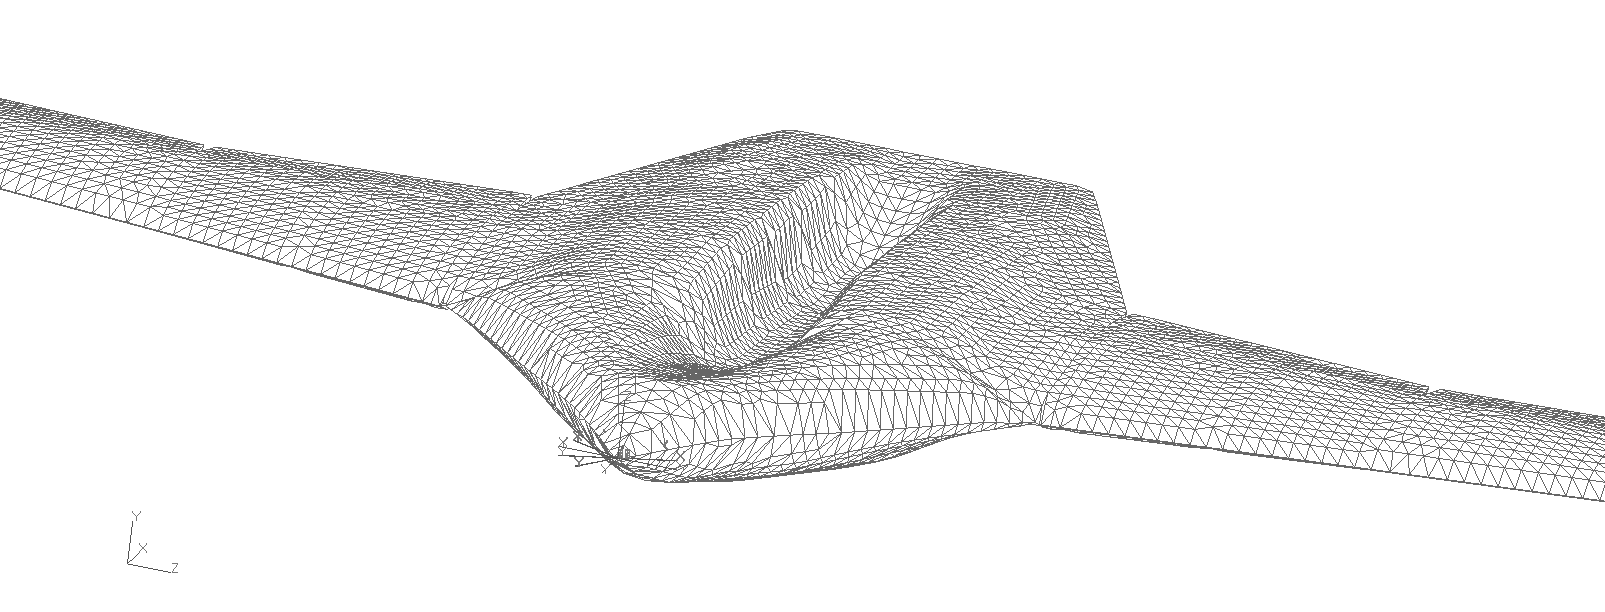
\includegraphics[width=0.9\textwidth]{BPLAfullModel}
\caption{МКЭ-модель гипотетической конструкции БПЛА}
\label{fig:fullMKE}
\end{figure}

\begin{figure}[ht]
\centering 
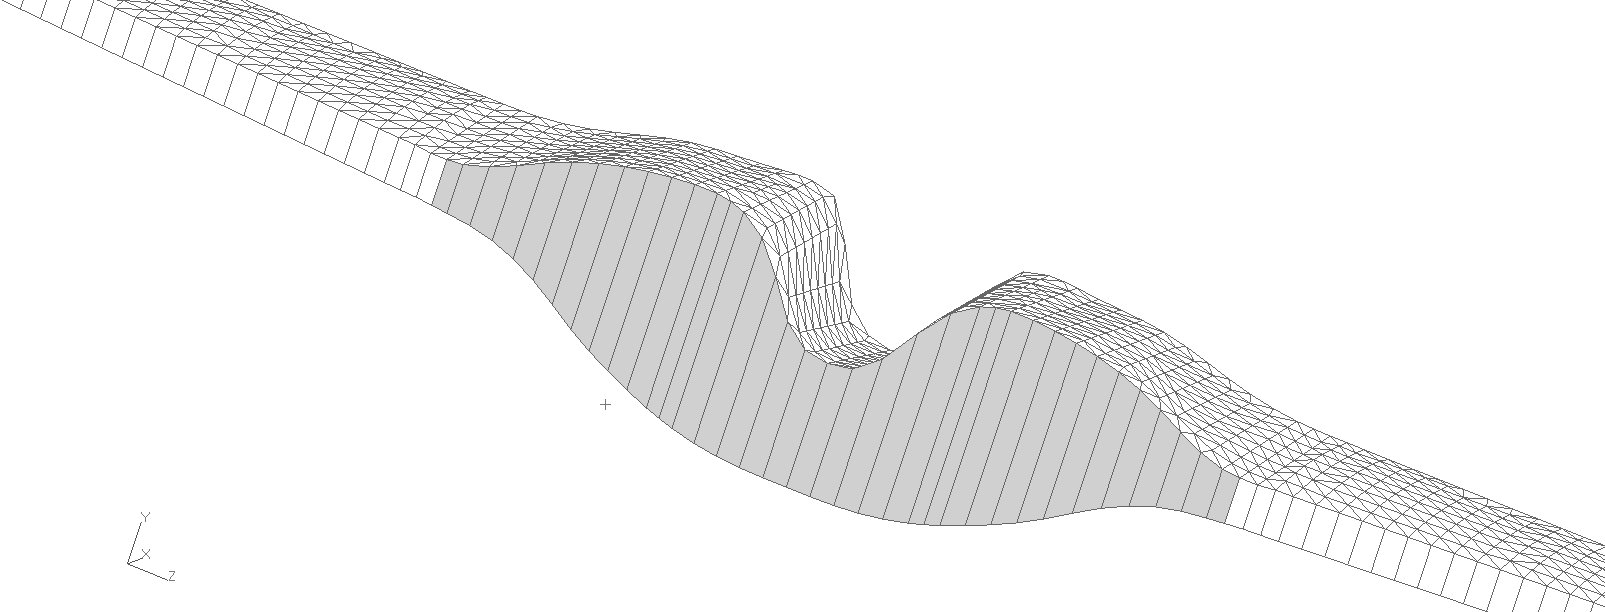
\includegraphics[width=0.9\textwidth]{centroplan}
\caption{МКЭ-модель центроплана гипотетической конструкции БПЛА}
\label{fig:centroplanMKE}
\end{figure}

\begin{figure}[ht]
\centering
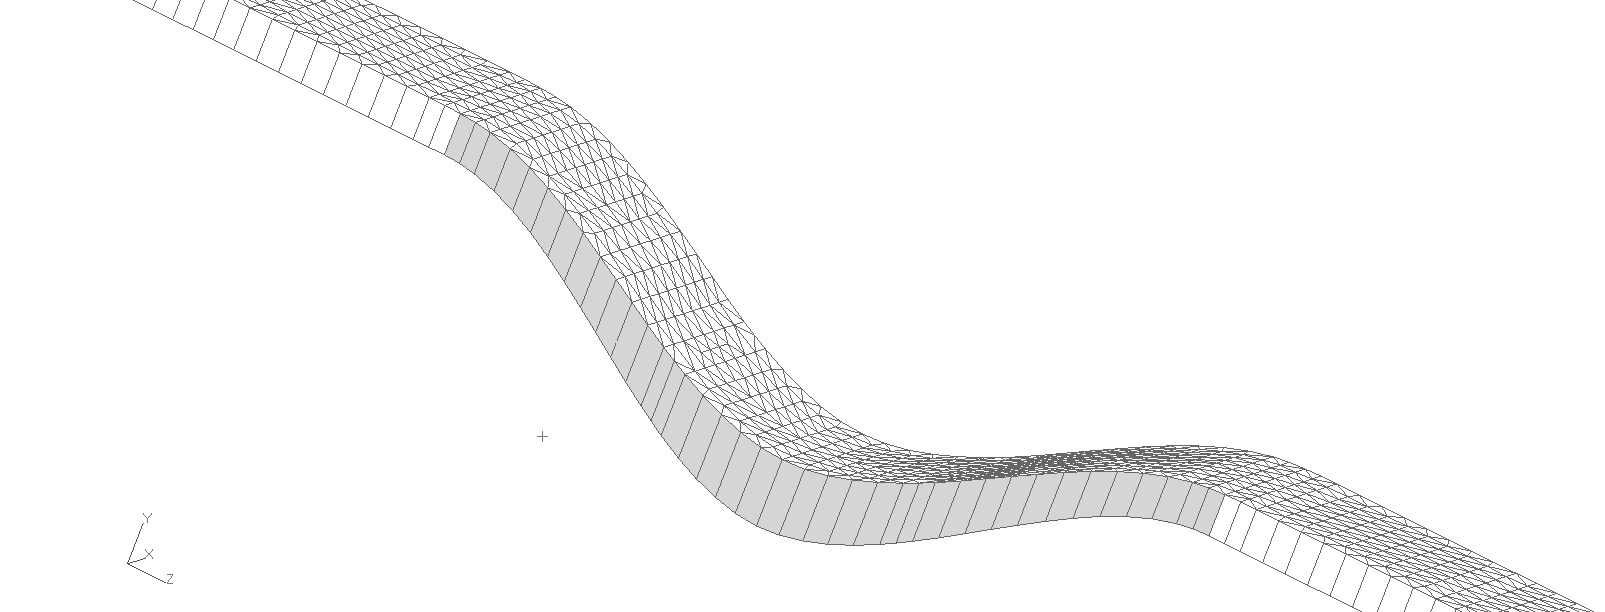
\includegraphics[width=0.9\textwidth]{simplifiedCentroplan}
\caption{Упрощенная модель центроплана}
\label{fig:simplifiedCentroplanMKE}
\end{figure}

Использование в МКЭ-расчете такой упрощенной модели позволяет значительно ускорить процесс прочностного параметрического анализа при тех же вычислительных мощностях. Так, в упрощенной модели используется $\approx10000$ конечных элементов, в то время как в полной модели самолета используется $\approx270000$ конечных элементов.

Как было сказано выше, рассматриваемая модель определяется двумя базовыми параметрами: координата нижней точки сечения относительно базовой горизонтали БПЛА $y_\text{отн}$ и строительная высота сечения в плоскости симметрии самолета $h_\text{стр}$. В качестве кривых, описывающих нижнюю и верхнюю поверхность кессона выбраны кубические сплайны, построенные через найденные исходя из выбранных параметров точки. Производные сплайнов в точках стыка фюзеляжа с крылом ($z=2.45\text{м}$) и в плоскости симметрии самолета ($z=0\text{м}$) приняты равными нулю. Пример модельного сечения центроплана в плоскости YZ со значениями параметров $h_\text{стр}=0.4\text{м}$, $y_\text{отн} = -1.4\text{м}$ приведен на Рис.\ref{fig:KessSectionExample}.

\begin{figure}[ht]
\centering
\def\svgwidth{\textwidth}
%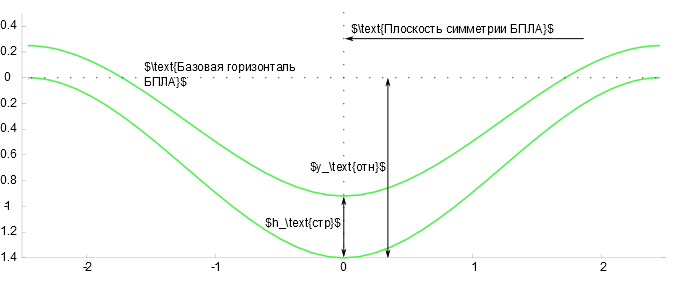
\includegraphics[width=1\textwidth]{KessSectionExample}
\input{figures/KessSectionExample.pdf_tex}
\caption{Пример формируемого параметрически поперечного сечения центроплана}
\label{fig:KessSectionExample}
\end{figure}

